\begin{problem}
试描述SOA三角操作模型,并对比传统的端到端服务调用模式,阐述其IT优势和商业优势。
\end{problem}

\begin{solution}
\begin{figure}[H]
    \vspace{-0.5em}
	\centering
	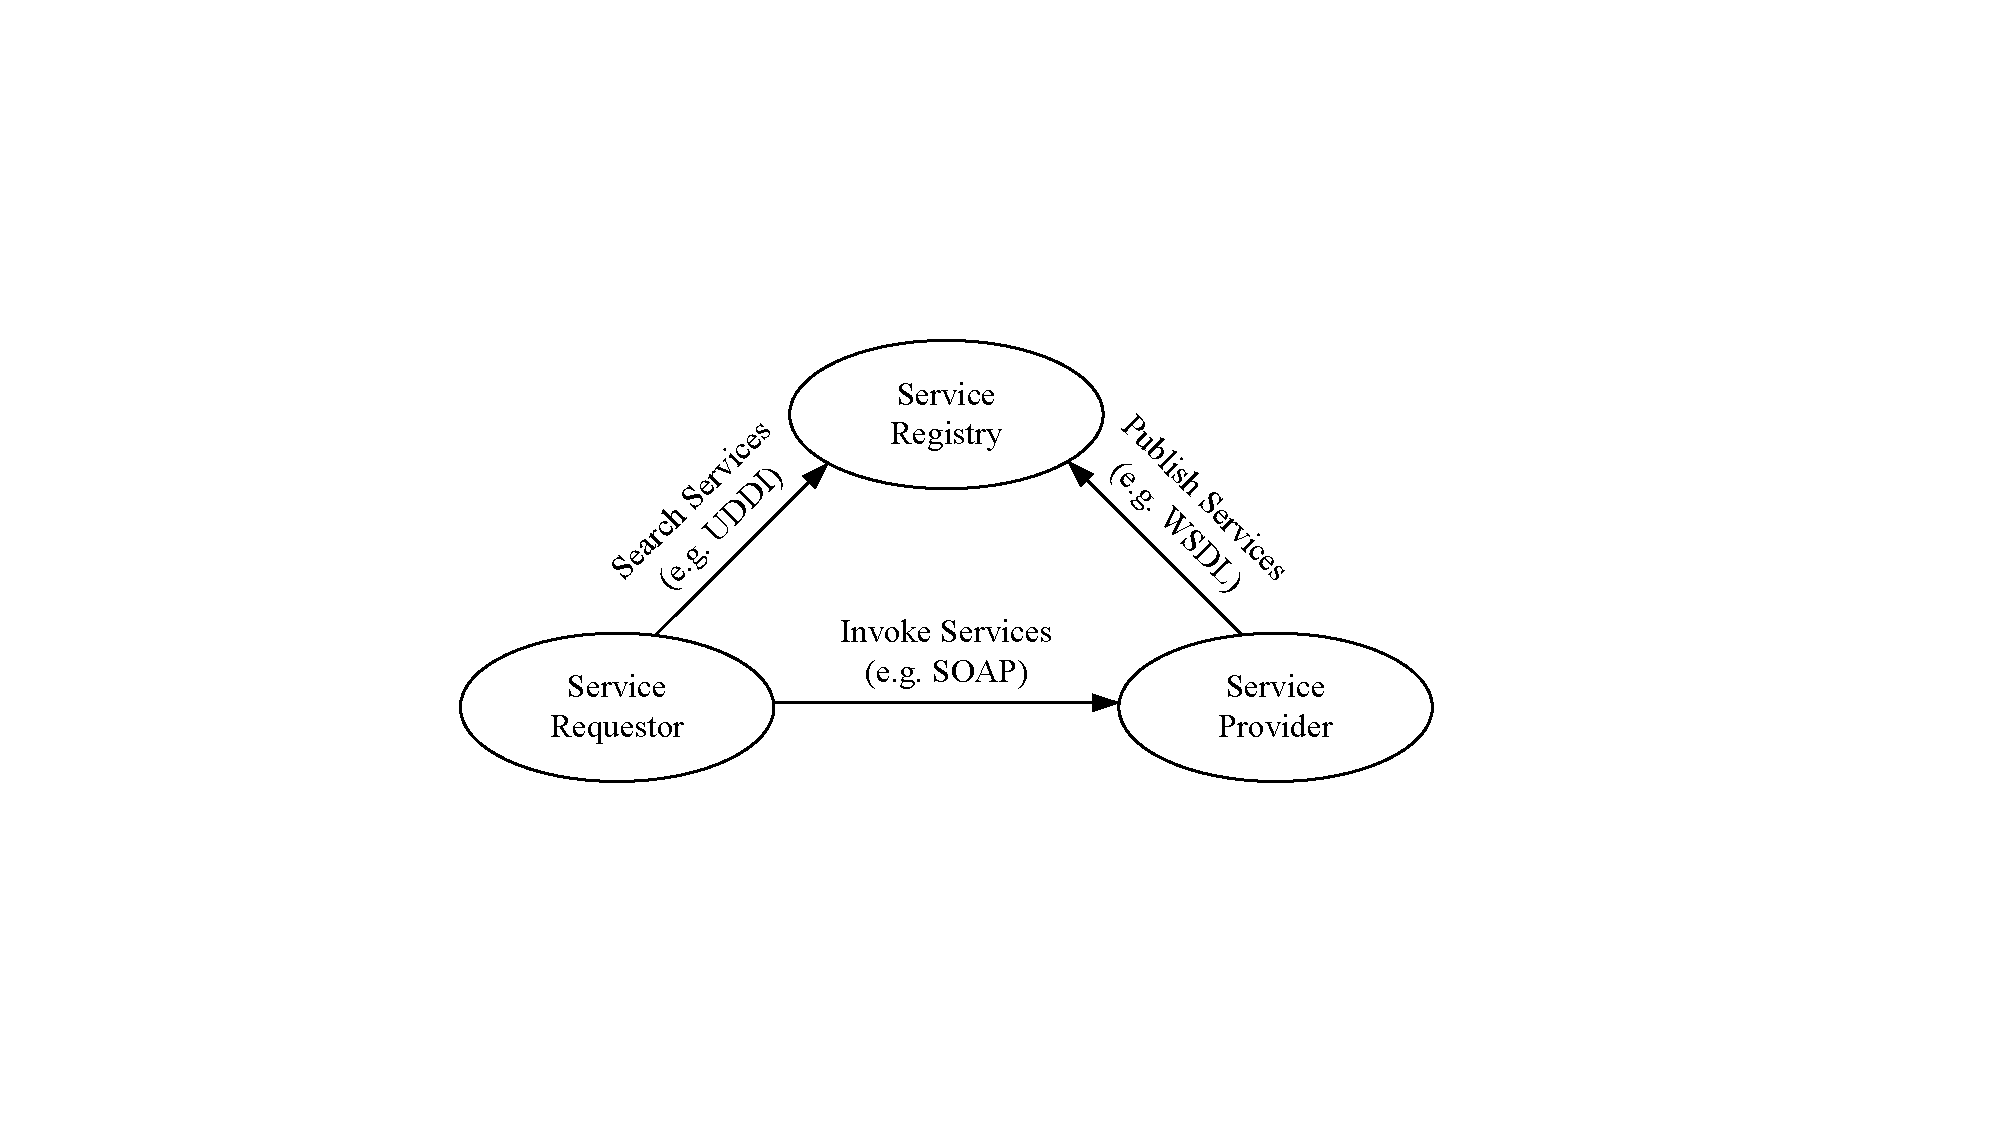
\includegraphics[width=0.5\textwidth]{SOA三角操作模型.pdf}
    \vspace{-1em}
\end{figure}

\begin{spacing}{1.2}
    \vspace{-0.5em}
    \begin{longtable}{|m{7.5cm}|m{7.5cm}|}
        \hline
        \multicolumn{1}{|c|}{\textbf{三种角色}} & \multicolumn{1}{c|}{\textbf{三个操作}} \\ \hline
        \vspace{-1.3em}
        \begin{itemize}[leftmargin=1.5em,itemsep=-3pt]
            \item 服务提供者:发布自己的服务,并且对服务请求进行响应
            \item 服务请求者:利用服务注册查找所需要的服务,然后使用该服务
            \item 服务注册商:注册已经发布的服务,对其进行分类,并提供搜索服务 
        \vspace{-1.5em}
        \end{itemize}                                           
            & 
        \vspace{-1.3em}
        \begin{itemize}[leftmargin=1.5em,itemsep=-3pt]
            \item 发布:为了使服务可访问,需要发布服务描述以使服务使用者可以发现它
            \item 查找:服务请求者查询服务注册来找到满足其标准的服务
            \item 绑定:检索到服务描述后,服务使用者继续根据服务描述中的信息调用服务
        \vspace{-1.5em}
        \end{itemize}  
        \\ \hline
    \end{longtable}
    \vspace{-1em}
\end{spacing}

SOA的优点:
\begin{spacing}{1.2}
    \vspace{-0.5em}
    \begin{longtable}{|m{7.5cm}|m{7.5cm}|}
        \hline
        \multicolumn{1}{|c|}{\textbf{IT优势}} & \multicolumn{1}{c|}{\textbf{商业优势}} \\ \hline
        \vspace{-1.3em}
        \begin{itemize}[leftmargin=1.5em,itemsep=-3pt]
            \item 松耦合,消除假依赖(复用):语言、平台和厂商中立;消除时间依赖;消除访问地址依赖;消除访问协议依赖
            \item 服务间接寻址(灵活)
        \vspace{-1.5em}
        \end{itemize}                                           
            & 
        \vspace{-1.3em}
        \begin{itemize}[leftmargin=1.5em,itemsep=-3pt]
            \item 保护企业投资,提升现有IT资源的作用,促进IT资源的复用
            \item 提高企业灵敏度
            \item 支持企业外包管理模式
        \vspace{-1.5em}
        \end{itemize}  
        \\ \hline
    \end{longtable}
    \vspace{-1em}
\end{spacing}

\end{solution}